\chapter{Metodologia}


\section{Descrição Geral}

O projeto consiste na concepção e implementação de uma nova plataforma de eventos para o Instituto Humanitas da Universidade, com o objetivo de modernizar e aprimorar significativamente o sistema atual. A plataforma será um ponto central para a divulgação e gerenciamento de eventos acadêmicos, culturais e científicos promovidos pelo instituto, proporcionando uma experiência mais intuitiva, atrativa e eficiente para toda a comunidade universitária.

O design da plataforma será cuidadosamente elaborado para refletir a identidade visual do Instituto Humanitas, garantindo uma interface moderna, limpa e atraente. Além disso, serão integrados recursos interativos, como calendário, notificações automáticas e estatísticas, para aumentar o engajamento e a participação da comunidade nos eventos.


\section{Especificações Técnicas}

\subsection{Banco de Dados}


\subsection{Front-End}


\subsection{Back-End}


\section{Descrição de Interfaces}


\section{Casos de uso}


\section{Diagrama de ER}

Abaixo está o diagrama de Entidade/Relacionamentos que ilustra a estrutura e os relacionamentos entre as entidades do sistema:

\begin{figure}[h]
\centering
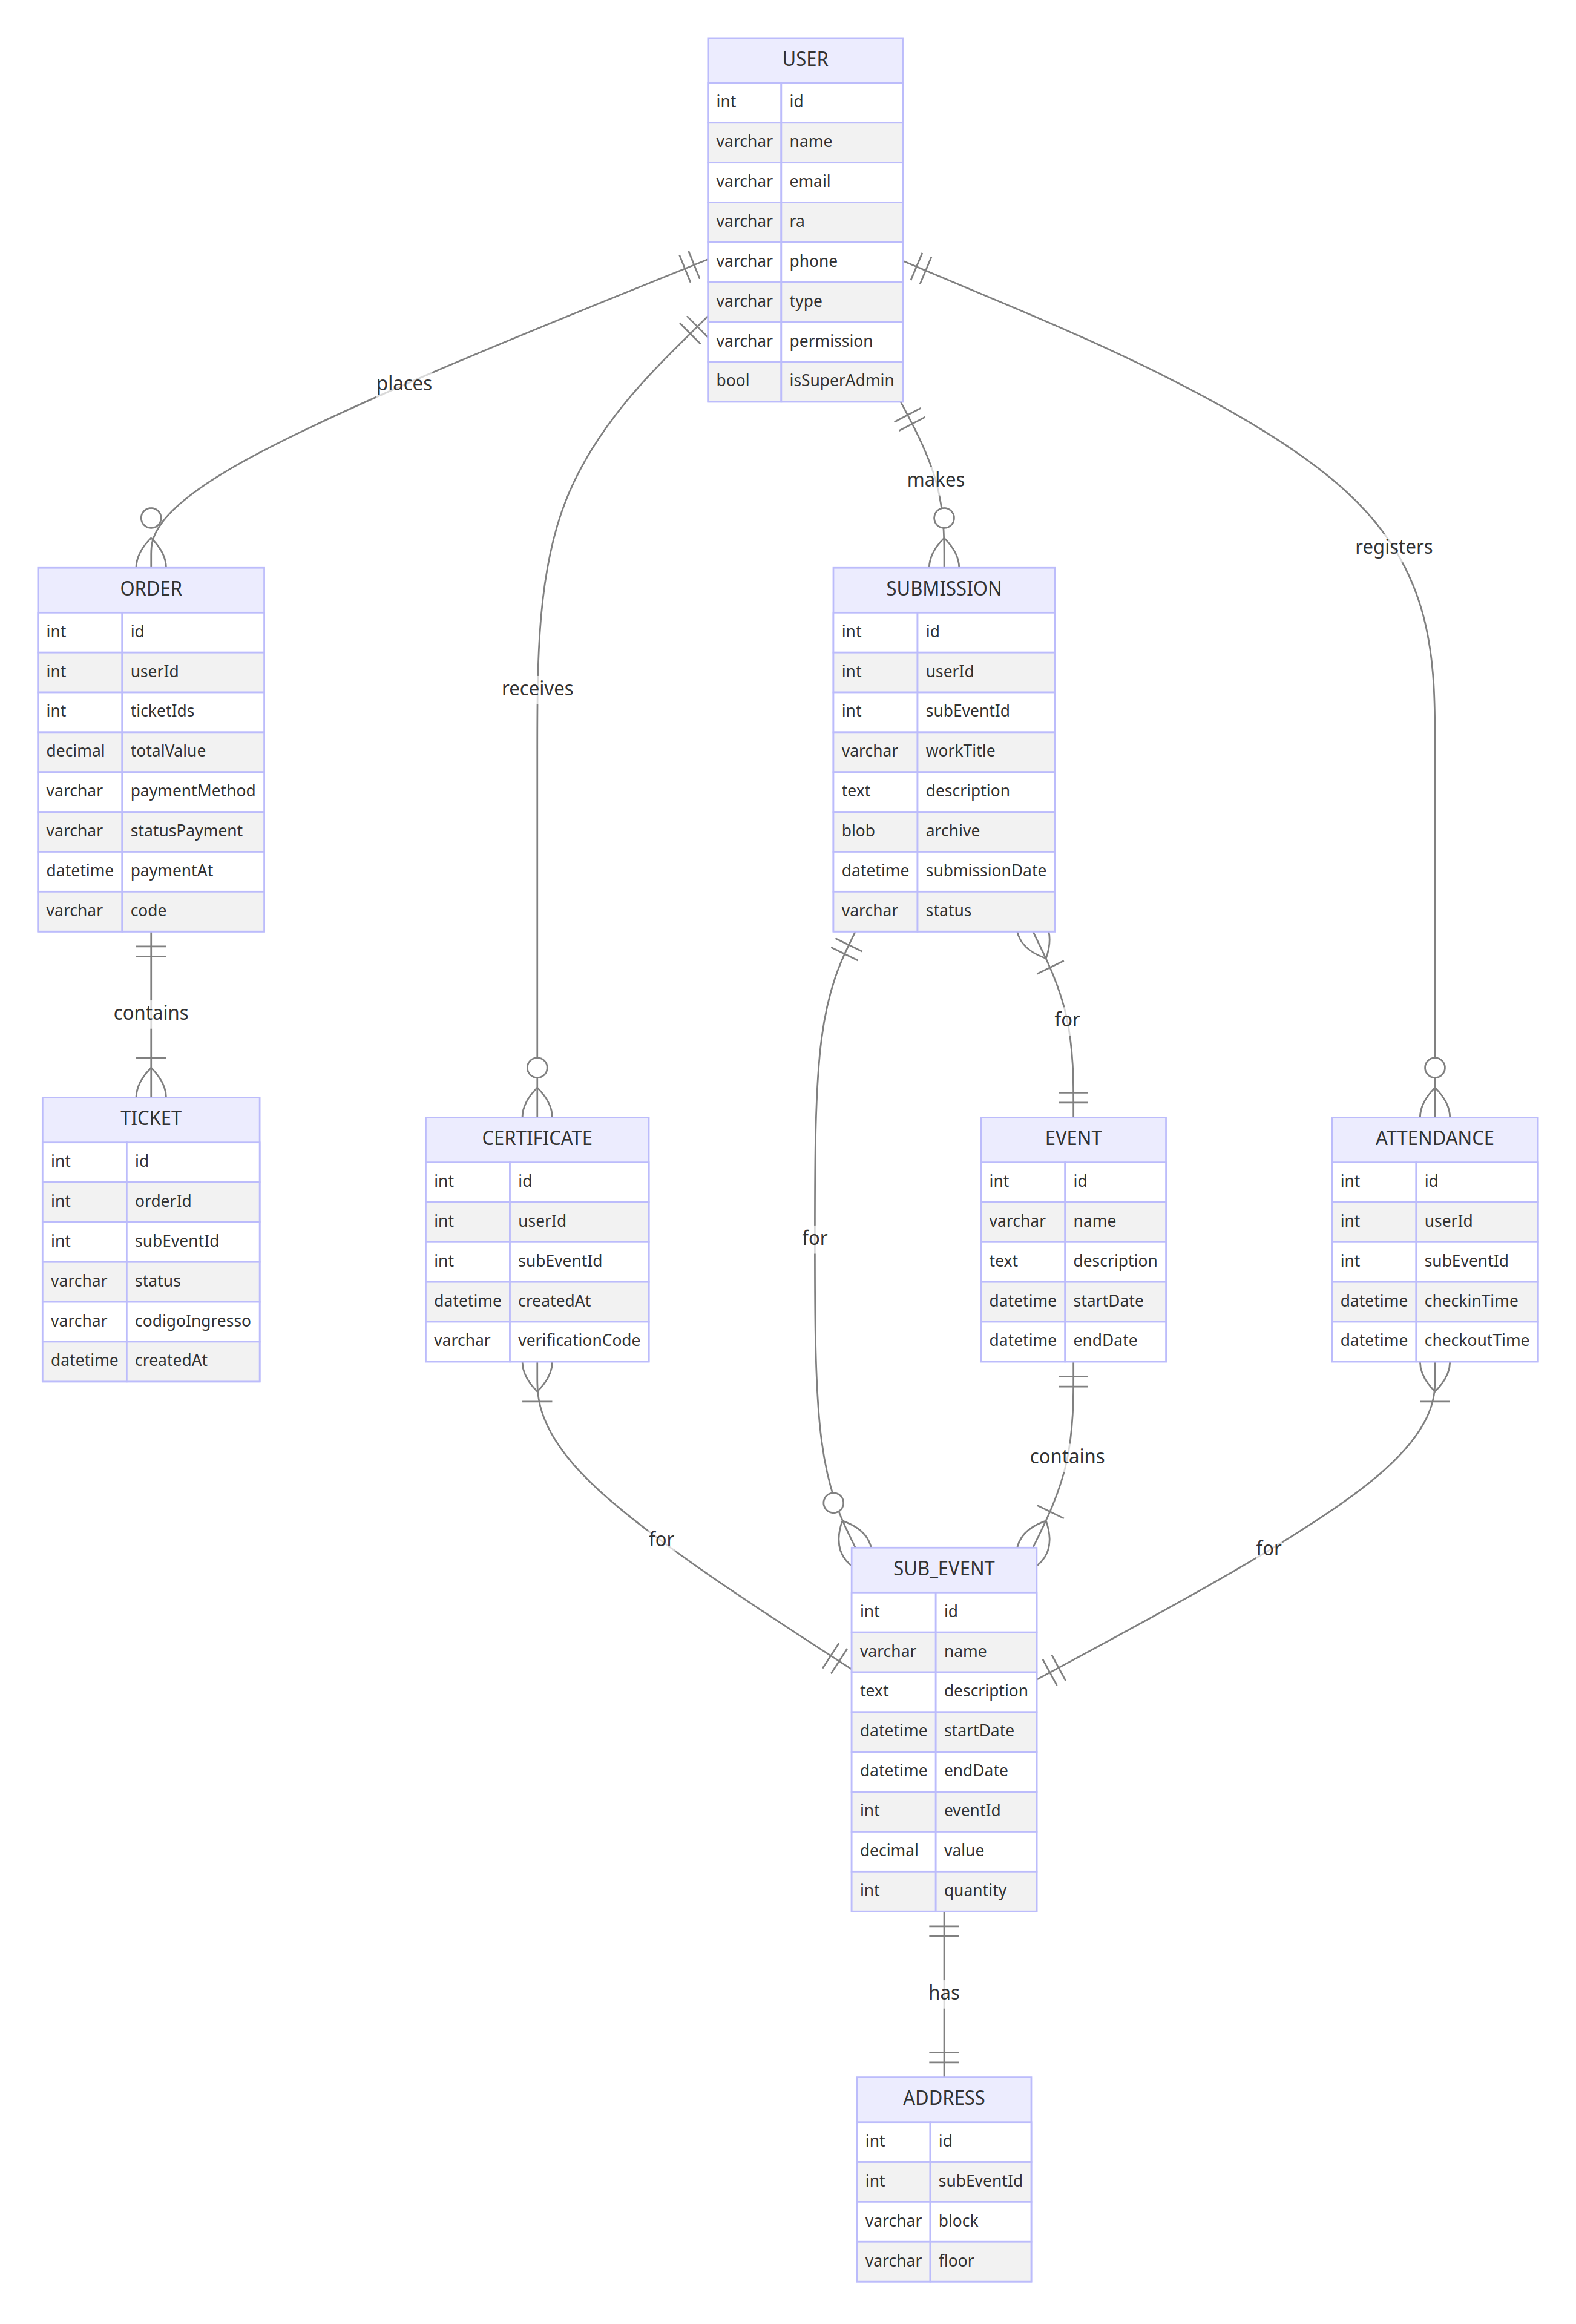
\includegraphics[width=0.8\textwidth]{figuras/diagrama-entidades.png}
\caption{Diagrama de Entidades do Sistema}
\label{fig:diagrama-entidades.png}
\end{figure}

\begin{verbatim}
erDiagram
    USER ||--o{ ORDER : places
    ORDER ||--|{ TICKET : contains
    USER ||--o{ CERTIFICATE : receives
    CERTIFICATE }|--|| SUB_EVENT : "for"
    USER ||--o{ SUBMISSION : makes
    SUBMISSION }|--|| EVENT : "for"
    SUBMISSION ||--o{ SUB_EVENT : "for"
    EVENT ||--|{ SUB_EVENT : contains
    SUB_EVENT ||--|| ADDRESS : has
    USER ||--o{ ATTENDANCE : registers
    ATTENDANCE }|--|| SUB_EVENT : "for"

    USER {
        int id
        varchar name
        varchar email
        varchar ra
        varchar phone
        varchar type
        varchar permission
        bool isSuperAdmin
    }

    ORDER {
        int id
        int userId
        int ticketIds
        decimal totalValue
        varchar paymentMethod
        varchar statusPayment
        datetime paymentAt
        varchar code
    }

    TICKET {
        int id
        int orderId
        int subEventId
        varchar status
        varchar codigoIngresso
        datetime createdAt
    }

    CERTIFICATE {
        int id
        int userId
        int subEventId
        datetime createdAt
        varchar verificationCode
    }

    SUBMISSION {
        int id
        int userId
        int subEventId
        varchar workTitle
        text description
        blob archive
        datetime submissionDate
        varchar status
    }

    EVENT {
        int id
        varchar name
        text description
        datetime startDate
        datetime endDate
    }

    SUB_EVENT {
        int id
        varchar name
        text description
        datetime startDate
        datetime endDate
        int eventId
        decimal value
        int quantity
    }

    ADDRESS {
        int id
        int subEventId
        varchar block
        varchar floor
    }

    ATTENDANCE {
        int id
        int userId
        int subEventId
        datetime checkinTime
        datetime checkoutTime
    }
\end{verbatim}